\documentclass[a4paper, 12pt, diplomski]{etfcyr}

\usepackage{fontspec}
\usepackage{polyglossia}
\usepackage[document]{ragged2e}
\usepackage{indentfirst}
\usepackage{enumitem}
\usepackage{scrextend}
\usepackage{etoolbox}
\usepackage{graphicx}
\usepackage{wrapfig}

\DeclareGraphicsExtensions{.pdf,.png,.jpg}

\addtokomafont{labelinglabel}{\textbf}

\setdefaultlanguage[script=Cyrillic]{serbian}
\newfontfamily{\cyrillicfont}{Times New Roman}

\setmainfont{Times New Roman}
\setsansfont{Arial}
\setmonofont{Courier New}

\renewcommand*\contentsname{Садржај}

\newcommand{\indentfirstparagraphon}{
    \renewenvironment{justify}{%
    	\trivlist
    	\justifying
    	\itemindent\JustifyingParindent
    	\item\relax
    }{
        \endtrivlist
    }
}

\newcommand{\indentfirstparagraphoff}{
    \renewenvironment{justify}{%
        \trivlist
        \justifying
        \item\relax
    }{
        \endtrivlist
    }
}

\makeatletter
\gdef\tshortstack{\@ifnextchar[\@tshortstack{\@tshortstack[c]}}
\let\@tshortstack\@shortstack
\patchcmd\@tshortstack\vbox\vtop{}{}
\makeatother

\indentfirstparagraphon

\addto\captionsserbian{%
  \renewcommand{\bibname}%
    {Литература}%
}

\setlength{\parindent}{4em}
\setlength{\JustifyingParindent}{4em}

\title{Паметна соба - контрола уласка} 
\author{Топлица Танасковић}
\indeks{164/1996}
\date{септембар 2016.}
\mentor{Саша Стојановић}
\predmet{Системско програмирање}

\begin{document}
	\sloppy
	\maketitle
	\begin{abstract}
		\begin{justify}
			У овом раду је изложен проблем прављења распореда коришћења лабораторија са контролом уласка. Објашњени су најчешћи сценарији који задају доста проблема и предложено је софтверско решење.
		\end{justify}
	\end{abstract}

	\begin{keywords}
		Дипломски радови, контрола приступа, програмирање, C++
	\end{keywords}
	\tableofcontents
	\listoffigures
	\listoftables

	\chapter{Увод}
		
		\section{Опис проблема}
		
		\begin{justify}
			Прављење распореда рада у факултетским лабораторијама је велики проблем са којим особље мора стално да се носи. Број студената и актвности које морају да се обаве је огроман, а факултет има ограничен број и лабораторија и радних места у њима. Ово представља проблем за људе који су одговорни за прављење распореда пошто морају да воде рачуна о много активности, студената и временских слотова док у исто време покушавају да избегну преклапања или конфликте.
		
			Проблем можемо сагледати са два аспекта, први је прављење распореда, а други је безбедност. Како је већ напоменуто, факултет има ограничен број лабораторија одређеног капацитета док је број студената са својим задацима и обавезним активностима огроман.
		
			Прављење распореда рада са дозволом уласка је врло тешко јер захтева праћење великог броја, како студената, тако и активности како би се обезбедило да нема преклапања. Радити ово ручно није оптимално и подложно је грешкама што може да доведе до разних преклапања, промена распореда у задњи час и многих других проблема. Без обзира што многе активности нису обавезне доста активности је у исто време и обавезно и врло битно за студенте, као што су рецимо колоквијуми или испити. Овакве активности не би смеле да се одлажу нити прекидају улажењем других особа у просторију.
		
			Што се тиче безбедности, неке лабораторије осим што имају деликатну и скупу, имају и врло опасну опрему која може услед погрешног руковања да начини огромну штету или чак нанесе опасне повреде. Због овога би требало ограничити приступ тј. улаз у неке од лабораторија како би се избегле у крајњим случајевима и несагледиве последице.
		\end{justify}

	\chapter{Дискусија}
		
		\section{Начини коришћења лабораторија}
		
		\begin{justify}
			Број начина на које једна лабораторија може да се користи углавном зависи од њене намене. Међутим, без обзира на намену лабораторије могу се уочити четири најчешћа начина на које се оне користе. Да би се целокупан проблем прецизније дефинисао, у овом одељку ће се дискутовати понаособ сваки од начина коришћења.
		\end{justify}
		
		\subsection{Дефиниције}
		
		\begin{justify}
			Пре него што будемо могли да опишемо начине на које се лабораторије користе, морамо увести неке дефиниције и успоставити релације између њих.
		\end{justify}


   		\begin{labeling}{\smash{\tshortstack[l]{Корисник\\лабораторије}}}
            \indentfirstparagraphoff            
            
            \item [Активност] 
                \begin{justify}
                    Активност је било који процес који се одвија у лабораторији, без обзира на његово трајање, евентуалну периодичност или конкретан тип.
                \end{justify}

            \item[\smash{\tshortstack[l]{Тип\\активности}}]
                \begin{justify}
                   Тип активности ближе дефинише активност, и одређује њен приоритет у односу на друге. Постоје следећи типови активности.
                   \begin{enumerate}[noitemsep]
                       \item Испит
                       \item Колоквијум
                       \item Предавања или вежбе
                       \item Лабораторијске вежбе
                       \item Посебни догађаји
                       \item Индивидуални рад
                    \end{enumerate}
                \end{justify}

            \item[\smash{\tshortstack[l]{Приоритет\\активности}}]
                \begin{justify}
                Приоритет активности одређује да ли је дозвољен улаз у просторију уколико се у њој преклапају активности, а једна од њих је битнија. Не желимо да допустимо да људи улазе и излазе из просторије док је у току испит. Приоритет активност је дефинисан типом активности како је наведено у претходној дефиницији.

                \indent Индивидуални рад је посебан случај. Приликом заказивања такве активности може се посебно дозволити улазак без обзира на то да ли се у просторији већ одвија нека активност вишег приоритета. Ово се углавном користи за студенте који раде дипломски или неки други важан пројекат.
                
                \end{justify}


            \item[\smash{\tshortstack[l]{Корисник\\лабораторије}}]
                \begin{justify}
                    Корисник лабораторије је било која особа којој се може дозволити улаз у лабораторију. Постоје две врсте корисника:
                    \begin{enumerate}[noitemsep]
                        \item Професор
                        \item Студент
                    \end{enumerate}
                    Можда би се могао увести и студент демонстратор као засебан тип корисника, али како он нема посебна права, довољно је да буде члан листе како би могао да приступи лабораторији.
                \end{justify}
            
            \item [Листа]
                \begin{justify}
                    Листе су групе особа-корисника лабораторија које служе зарад лакше манипулације током заказивања активности и доделе права уласка у лабораторију.
                    \begin{enumerate}[noitemsep]
                        \item Системске листе
                        \item Трајне листе
                        \item Привремене листе
                    \end{enumerate}
                    Привремене листе имају свој рок трајања и након тога се аутоматски бришу из система. Системске листе су посебан случај трајних листа, оне се не могу мењати и о њима систем сам води рачуна. Пример системске листе је листа студената друге године.
                \end{justify}
            
            \item [Просторија]
                \begin{justify}
                    Просторија је било која лабораторија, кабинет или учионица у којој се одвијају неке активности у за коју желимо да имамо контролу уласка.
                \end{justify}
            
            \indentfirstparagraphon
    	\end{labeling}
        
        \subsection[Сценарио 1]{Испити и колоквијуми}
            \begin{justify}
                Ово је вероватно најбитнији сценариo. Активности дефинисане овим сценариом се обично не понављају и имају тачно дефинисан датум и време почетка као и трајање. Оваквим активностима се обично додељује искључиво једна листа студената, али није искључено да се доделе и више. Такође овакве активности се најчешће одвијају у више просторија паралелно
            \end{justify}
        
        \subsection[Сценарио 2]{Предавања или вежбе}
            \begin{justify}
                Предавања и вежбе су пример активности која се понавља на недељном нивоу један дужи временски период, и одвијају се у једној просторији. Ову врсту активности обично посећује иста група људи, прецизније студенти који слушају дати предмет или ако је предмет обавезан онда сви студенти дате године студија.
            \end{justify}
        
        \subsection[Сценарио 3]{Лабораторијске вежбе}
            \begin{justify}
                Лабораторијске вежбе су пример активности код којих поред студената и професора можемо имати и студенте демонстраторе. Студентима демонстраторима би требало такође дозволити несметан улаз и то се лако може постићи додавањем нове листе која ће садржати демонстраторе у систем, и додељивањем те листе активности. Овакве активности се најчешће изводе у једној просторији, али није немогуће да се одвијају паралелно у више.
            \end{justify}
        
        \subsection[Сценарио 4]{Посебни догађаји}
            \begin{justify}
                У овакве активност превасходно спадају јавна предавања, презентације и конференције. У оваквим случајевима у простиријама се увек налази неко од особља као што су предавачи, контрола приступа није потребна. Овакве активности не захтевају да имају додељену листу.
            \end{justify}
        
        \subsection[Сценарио 5]{Индивидуални рад}
            \begin{justify}
                Код ове врсте активност специфично је то што она може, ако је дефинисано, да дозволи улаз у просторију без обзира да ли је нека друга активност у току. Оваква активност захтева листу студената, којој може да припада и само један студент. Овакве активности се најчешће одобравају студентима који раде дипломски или неки други важан рад, а имају потребу за опремом која се налази у лабораторијама.
            \end{justify}
            
        \section{Посебне напомене}
            \begin{justify}
                Уколико је неопходно, могуће је одређеним студентима забранити улазак у неку просторију. Студенти којима је улаз забрањен неће моћи да уђу у дату просторију иако су на листи за активност која се одвија у њој.
            \end{justify}
            
    \chapter{Предлог решења}
    
        \section{Уопштени преглед система}
            \begin{justify}
                Услед саме природе проблема, као и потребе да компоненте комуницирају на поуздан и безбедан начин, систем мора да буде модуларан са прецизно дефинисаним протколима комуникације и обраде грешака. Уопштен дијаграм система дат је на слици испод.\newline
                
                \begin{figure}[h]
                    \begin{center}
                        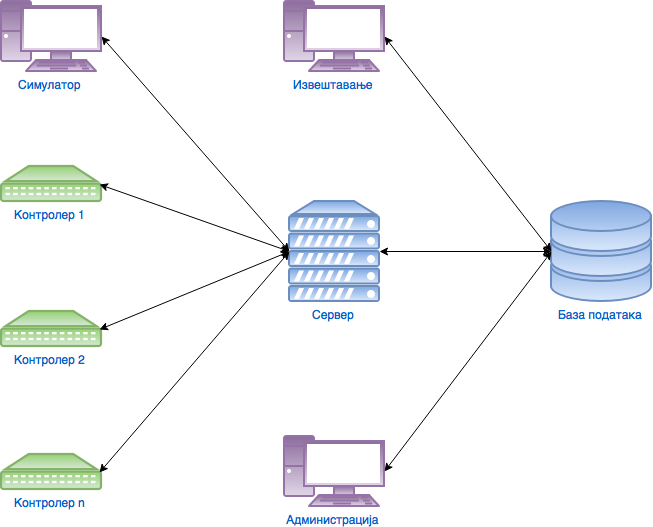
\includegraphics[scale=0.45]{SystemOverview.png}
                    \end{center}
                    \caption{Дијаграм система}
                \end{figure}
                
                На претходном дијаграму лако можемо уочити да постоје три различите врсте компоненти. Плаве су чисто софтверске компоненте које раде на серверу, љубичасте су такође софтверске компоненте, али раде на локалним рачунарима, док су зелене компоненте представљају микроконтролере са припадајућом хардверсо-софтверском подршком.
            \end{justify}
         
         \section{Компоненте система}
             
             \subsection{База података}
                 \begin{justify}
                     Сервер базе података је одговоран за свеобухватно похрањивање података. Посебних хардверских захтева нема, сем да постоји довољно меморије и складишног простора на диску. Сервер базе података који се користи у овом решењу је PostgreSQL издање 9.2, а може се користити и новија верзија.
                     \begin{figure}[h]
                         \begin{center}
                             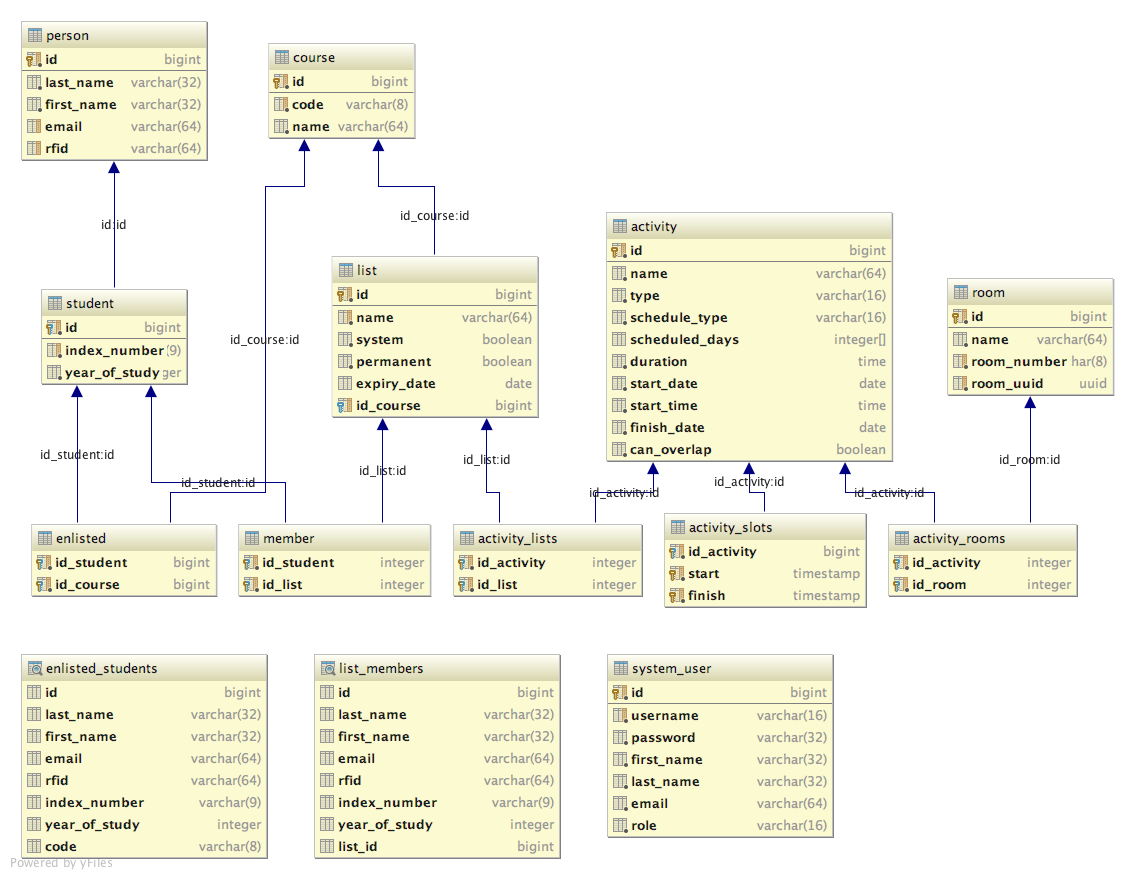
\includegraphics[scale=0.35]{DatabaseDiagram.png}
                         \end{center}
                         \caption{Дијаграм базе података}
                     \end{figure}
                 \end{justify}
                 
             \subsection{ПаСо Сервер}
                 \begin{justify}
                     ПаСо сервер је централна компонента система. Његова одговорност је да комуницира са контролерима просторија и са симулатором као алатом за тестирање. Сам сервер је имплементиран као стандардни UNIX димон који прихвата TCP конекције на порту који је одређен подешавањима. Овај сервер није пасивна компонента која само чека захтеве и обрађује их, већ периодично шаље и ”јеси ли жив” сигнале пријављеним контролерима и симулаторима. Такође, одговоран је и за слање података које би контролери требало да користе уколико дође до прекида у комуникацији. Формат комуникације, порука и података за случај прекида саме комуникације биће дефинисан касније.
                     
                     Илустрација рада сервера дата је на следећем дијаграму.
                     \begin{figure}[h]
                         \begin{center}
                             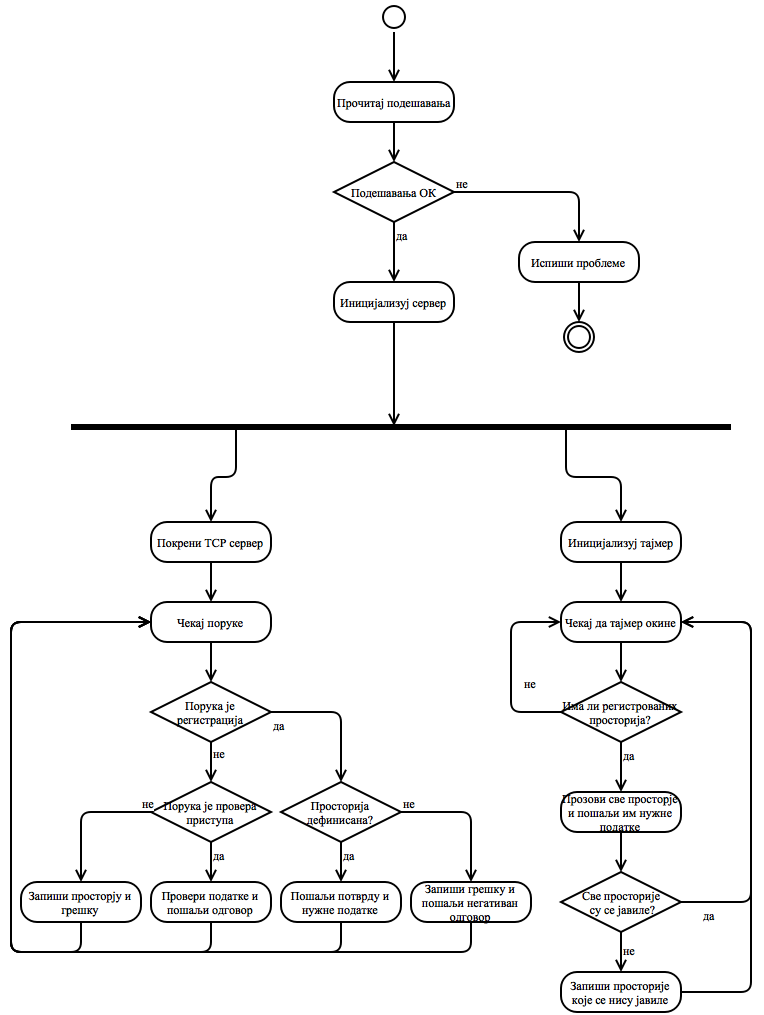
\includegraphics[scale=0.30]{ServerWorkflow.png}
                           \end{center}
                           \caption{Дијаграм рада сервера}
                       \end{figure}
                 \end{justify}
                 
             \subsection{Администрација}
                 \begin{justify}
                     Ова компонента је одговорна за комплетну администрацију целог система, почев од управљања корисницима и просторијама па све до заказивања активности.
                 \end{justify}
\end{document}